\apendice{Game Design Document}
\label{ap:game-design-document}


\section {Introducão}
\label{ap:introducao}

Este documento visa informar aspectos conceituais e artísticos do jogo Caapora RPG. O intuito do documento é estabelecer um objetivo comum para o desenvolvimento do jogo, auxiliando em duvidas gerais que possam aparecer nas fases de implementação do jogo em questão.

\subsection {Conceito}

Caapora RPG é um jogo 2.5D, monojogador, de \textit{action}/RPG habituada no cenário que será a floresta Amazônica, onde o jogador incorpora o Caipora e junto com a Iara e o Boto cor-de-rosa precisam defender a floresta dos caçadores, lenhadores e mineradores.

\subsection {Gênero}
É um jogo no estilo \textit{Action}/RPG, ou seja, um RPG com elementos de ação. 

\subsection {Público Alvo}
O jogo destina-se a jogadores com faixa etária dos 5 aos 12 anos, pois se trata de um jogo infantil e educativo.

\subsection {Plataforma}
O jogo será desenvolvido para dispositivos móveis, em especial para \textit {smartphones}

\section {História e Narrativa}
\label{ap:historia-e-narrativa}

Descreve a história do jogo, buscando informar onde se passa o jogo e os principais personagens envolvidos.

\subsection{Enredo}
Após ter uma visão onde a floresta é destruída, o Caipora, Guardião da Floresta, decide deixar de ser uma lenda e passa a agir. Desde então ele tem como missão evitar tudo aquilo que prejudique a Floresta Amazônica, como queimadas, desmatamento, poluição, entre outros. Para isso, ele contará com a ajuda de alguns membros como a Iara e o Boto.

\subsection {Personagens}
Descreve em profundidade os protagonistas principais do jogo, assim como os secundários que serão aqueles que ajudaram o personagem principal de algum modo.

\subsubsection{Caipora}
Caipora é o protagonista do jogo. É um índio conhecido como o “guardião da floresta” devido ao seu lado protetor. Sua missão é proteger a floresta Amazônica e os animais que nela habitam de inimigos, como os caçadores, mineradores, lenhadores e empresários que buscam de alguma forma se aproveitar da riqueza que há nela. 

Ele possui um arco com flechas e devido a sua convivência com os animais adquiriu a habilidade de imita-los, com isso utiliza desses requisitos para atacar e amedrontar seus inimigos.

\subsubsection{Curupira}
Curupira é um personagem do jogo que poderá ser selecionado no lugar do Caipora. Ele é um habitante da mata de estatura pequena, possui cabelos avermelhados e seus pés são voltados para trás. Sua função é proteger árvores, plantas e animais. Ele possui uma lança e pode emitir sons e assovios agudos que amedrontam seus inimigos.

\subsubsection{Iara}
Iara é uma personagem do jogo que ajudará o Caipora em alguns dos seus objetivos. Ela é uma sereia que possui uma voz irresistível capaz de atrair quem se aproxima dela para o fundo do rio.

\subsubsection{Boto Cor de Rosa}
Boto cor-de-rosa é um personagem do jogo que ajudará o Caipora a combater os incêndios. Ele é um peixe que habita nos rios da floresta Amazônica. Possui uma habilidade que lhe permite lançar jatos de água



\section {GamePlay}
\label{ap:gameplay}
Descreve os desafios encontrados pelo jogador e os métodos usados para superá-los.

\subsection {Estruturas de Missões e desafios}
O jogo será dividido em 4 missões que serão divididas entre os cenários do jogo.

\subsubsection{Primeira Missão}
Alguns pontos da floresta estão pegando fogo. Com isso o jogador deverá percorrer um caminho até o rio e pegar baldes de água para apagar o fogo. O jogador poderá recorrer ao especial do boto cor-de-rosa que é um jato de água, entretanto esse especial após seu uso terá um tempo de resfriamento. A missão termina quando não houver mais árvores pegando fogo na floresta.

\subsubsection{Segunda Missão}
Os lenhadores estão cortando árvores em certo ponto da floresta. Nesta Missão o jogador deverá percorrer o caminho até o local e utilizar o poder do caipora de imitar os animais para amedrontar os lenhadores e expulsar eles do local, entretanto eles irão para um outro local da floresta e novamente o jogador terá que ir até eles e amedrontar até que eles desistam.

\subsubsection{Terceira Missão}
Alguns mineradores estão poluindo o rio. Com isso, o jogador deverá atacar os mineradores utilizando a lança ou o arco com flechas. Cada ataque terá um tempo de resfriamento. Nesta missão o jogador poderá recorrer a Iara para atrair os mineradores para dentro do rio.

\subsubsection{Quarta Missão}
Empresários querem derrubar algumas árvores e destruir o habitat dos índios com o intuito de construir um parque de diversões. Nesta missão o jogador terá a ajuda dos índios, eles percorrerão a floresta criando armadilhas para destruir qualquer tipo de maquinário.

\section {Entradas}
\label{ap:entradas}
O jogador utilizará os controles de toque. Através dele o jogador poderá escolher as opções de tela inicial, como Jogar, Personagem, opções e até mesmo jogar.

\subsection {Controle}
Com os comandos de toque é possível movimentar o personagem em seu percurso e também executar ações, conforme ilustrado na figura 34.

\begin{figure}[h!]
		\centering
		\Caption{\label{fig:exemplo-1} Controles de movimentação e ação do personagem.}	
		\UECEfig{}{
			\fbox{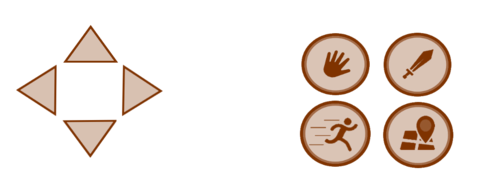
\includegraphics[width=13cm]{figuras/comandos}}
		}{
			\Fonte{Elaborado pelo autor}
		}	
	\end{figure}

\begin{alineascomponto}

	\item O botão 
\includegraphics[scale=0.5]{figuras/cima} move o personagem para cima.\\
	
	\item O botão 
\includegraphics[scale=0.5]{figuras/baixo} move o personagem para baixo.\\
	
	\item O botão 
\includegraphics[scale=0.5]{figuras/esquerda} move o personagem para a esquerda.\\ 
	
	\item O botão 
\includegraphics[scale=0.5]{figuras/direita} move o personagem para a direita.\\
	
	\item O botão com ícone 
\includegraphics[scale=0.5]{figuras/mao} pega objetos no chão.\\
	
	\item O botão com ícone 
\includegraphics[scale=0.5]{figuras/espada} lança objetos.\\
	
	\item O botão com ícone 
\includegraphics[scale=0.5]{figuras/mapa} faz com que todo o cenário fique visível.\\
	
	\item O botão com ícone 
\includegraphics[scale=0.5]{figuras/homen} faz com que o personagem corra.
	
\end{alineascomponto}

\section {Universo do Jogo}
\label{ap:universo-do-jogo}

\subsection {Cenário}

O jogo está dividido em quatro cenários que serão construídos tendo como base o mapa isométrico, conforme ilustra a figura 35.



\begin{figure}[h!]
		\centering
		\Caption{\label{fig:exemplo-1} Ilustração do Cenário}	
		\UECEfig{}{
			\fbox{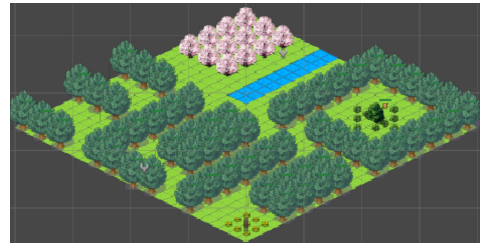
\includegraphics[width=13cm]{figuras/cenario}}
		}{
			\Fonte{Elaborado pelo autor}
		}	
	\end{figure}

Os cenários serão interligados através de portais, que poderão ser utilizados sempre que o personagem concluir uma missão.


